%
% In this file, we test the nohints option and the \useHints
%
\documentclass{article}
\usepackage{amsmath}
\usepackage{graphicx}
% Use these three for onscreen presentation.
\usepackage[tight,rightpanel]{web} %,usetemplates,rightpanel,leftpanel
\usepackage{exerquiz}
\usepackage[memLogo,nohints]{ecards}

% Use these three to get a listing of all questions, hints, and answers; useful
% for checking your work.
%\usepackage[forpaper,tight]{web} %  ,usetemplates
%\usepackage[solutionsafter,proofing]{exerquiz}
%\usepackage[memLogo,listing]{ecards}

% begin Web commands
\margins{.25in}{.25in}{24pt}{.25in} % left,right,top, bottom
\screensize{3.72in}{366.24bp}
\subject{Electronic Flash Cards}
\keywords{Flash Cards, LaTeX, PDF}
\university{THE UNIVERSITY OF AKRON\\
   Theoretical and Applied Mathematics}
\email{dpstory@uakron.edu}
\version{2.0}
\copyrightyears{\the\year}
\author{D. P. Story}
\title{The U.S. Presidents by Number\texorpdfstring{\\}{,} Numbers 1--6}

\norevisionLabel

\definecolor{logoblue}{rgb}{0,0,0.267}
\panelBgColor{logoblue}

\renewcommand\hproportionwebtitle{.9}

\newcommand\aebLogo{\parbox{1.75in}{\large \color{red}\textsl{eCards: U.S. Presidents}\\
    \small\smash{\raisebox{3pt}{\color{blue}\textsl{Acro\!\TeX{} eDucation Bundle}\hfill}}}}

\makeatletter
\ifecListing\else
    \ifnum\@panelconfig>0\relax
        \optionalPageMatter{\par\minimumskip\vspace{\stretch{1}}
            \begin{center}
            \fcolorbox{blue}{webyellow}{
            \begin{minipage}{.85\linewidth}
            \textbf{\textcolor{red}{Instructions:}}
            Click on the \textcolor{webblue}{Begin} button to view the
            first randomly selected card. Click on \textcolor{webblue}{FS} to view
            the flash cards in full screen mode (works only outside a web browser). The
            \textcolor{webblue}{Home} button on the first page goes to the
            \textbf{\textcolor{red}{Acro\!\TeX}} home page; otherwise, the
            \textcolor{webblue}{Home} button returns to this page.
            The \textcolor{webblue}{Close} button closes the document (use
            outside a web browser).\par\smallskip
            \textbf{\textcolor{red}{Source:}}
            \href{http://www.whitehouse.gov/history/presidents/}%
                {The White House Presidents Page}\par\smallskip
            \end{minipage}}
            \end{center}
        }
    \else
        \optionalPageMatter{\par\minimumskip\vspace{\stretch{1}}
            \begin{center}
            \fcolorbox{blue}{webyellow}{
            \begin{minipage}{.67\linewidth}
            Click on the \textcolor{webblue}{Begin} button to view the
            first randomly selected card.  Click  on
            \textcolor{webblue}{FS} to put the viewer into full screen
            mode (use outside a web browser). The check box on the
            right toggles the delivery of the cards between random
            and natural order; a check means random
            order.\par\smallskip
            \centering
                \Begin\ \FullScreen\ \ToggleOrder
            \end{minipage}}
            \end{center}
        }
    \fi
\fi
\makeatother
% end Web commands

% begin ecards commands
\ecLogoLink{http://www.uakron.edu/}
\cardsFinishedMsg{You've seen all the Presidents, at least the ones presented
    in these cards.}
\renewcommand\noHintJSAction{app.alert("No hint provided for this question!")}
% end ecards commands

\def\rescale{.4} % common re-scaling parameter for presidents
\parindent0pt


\begin{document}

\maketitle

\ifecListing
    \begin{center}\Large\bfseries
        Listing of Questions, Hints, and Answers
    \end{center}\bigskip
\fi

% This card should have no hint, which is the default with the nohints option
\begin{card}
    Who was the first President of the United States?
    \begin{response}
        \begin{hint}
            Legend has it, he chopped down the cherry tree and couldn't tell a lie.
        \end{hint}
        \begin{answer}
        \ifecListing
            George Washington (1789-1797)
        \else\centering
            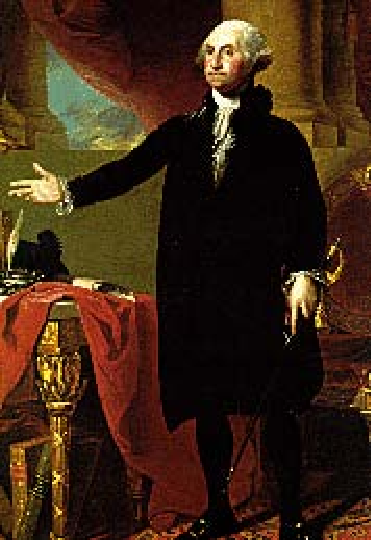
\includegraphics[scale=\rescale]{presidents/gw1}\\
                George Washington\\
                1789-1797
        \fi
        \end{answer}
    \end{response}
\end{card}

% Start using hints by default
\useHints

\begin{card}
    Who was the second President of the United States?
    \begin{response}
        \begin{hint}
            He was Washington's Vice President.
        \end{hint}
        \begin{answer}
        \ifecListing
            John Adams (1797-1801)
        \else\centering
            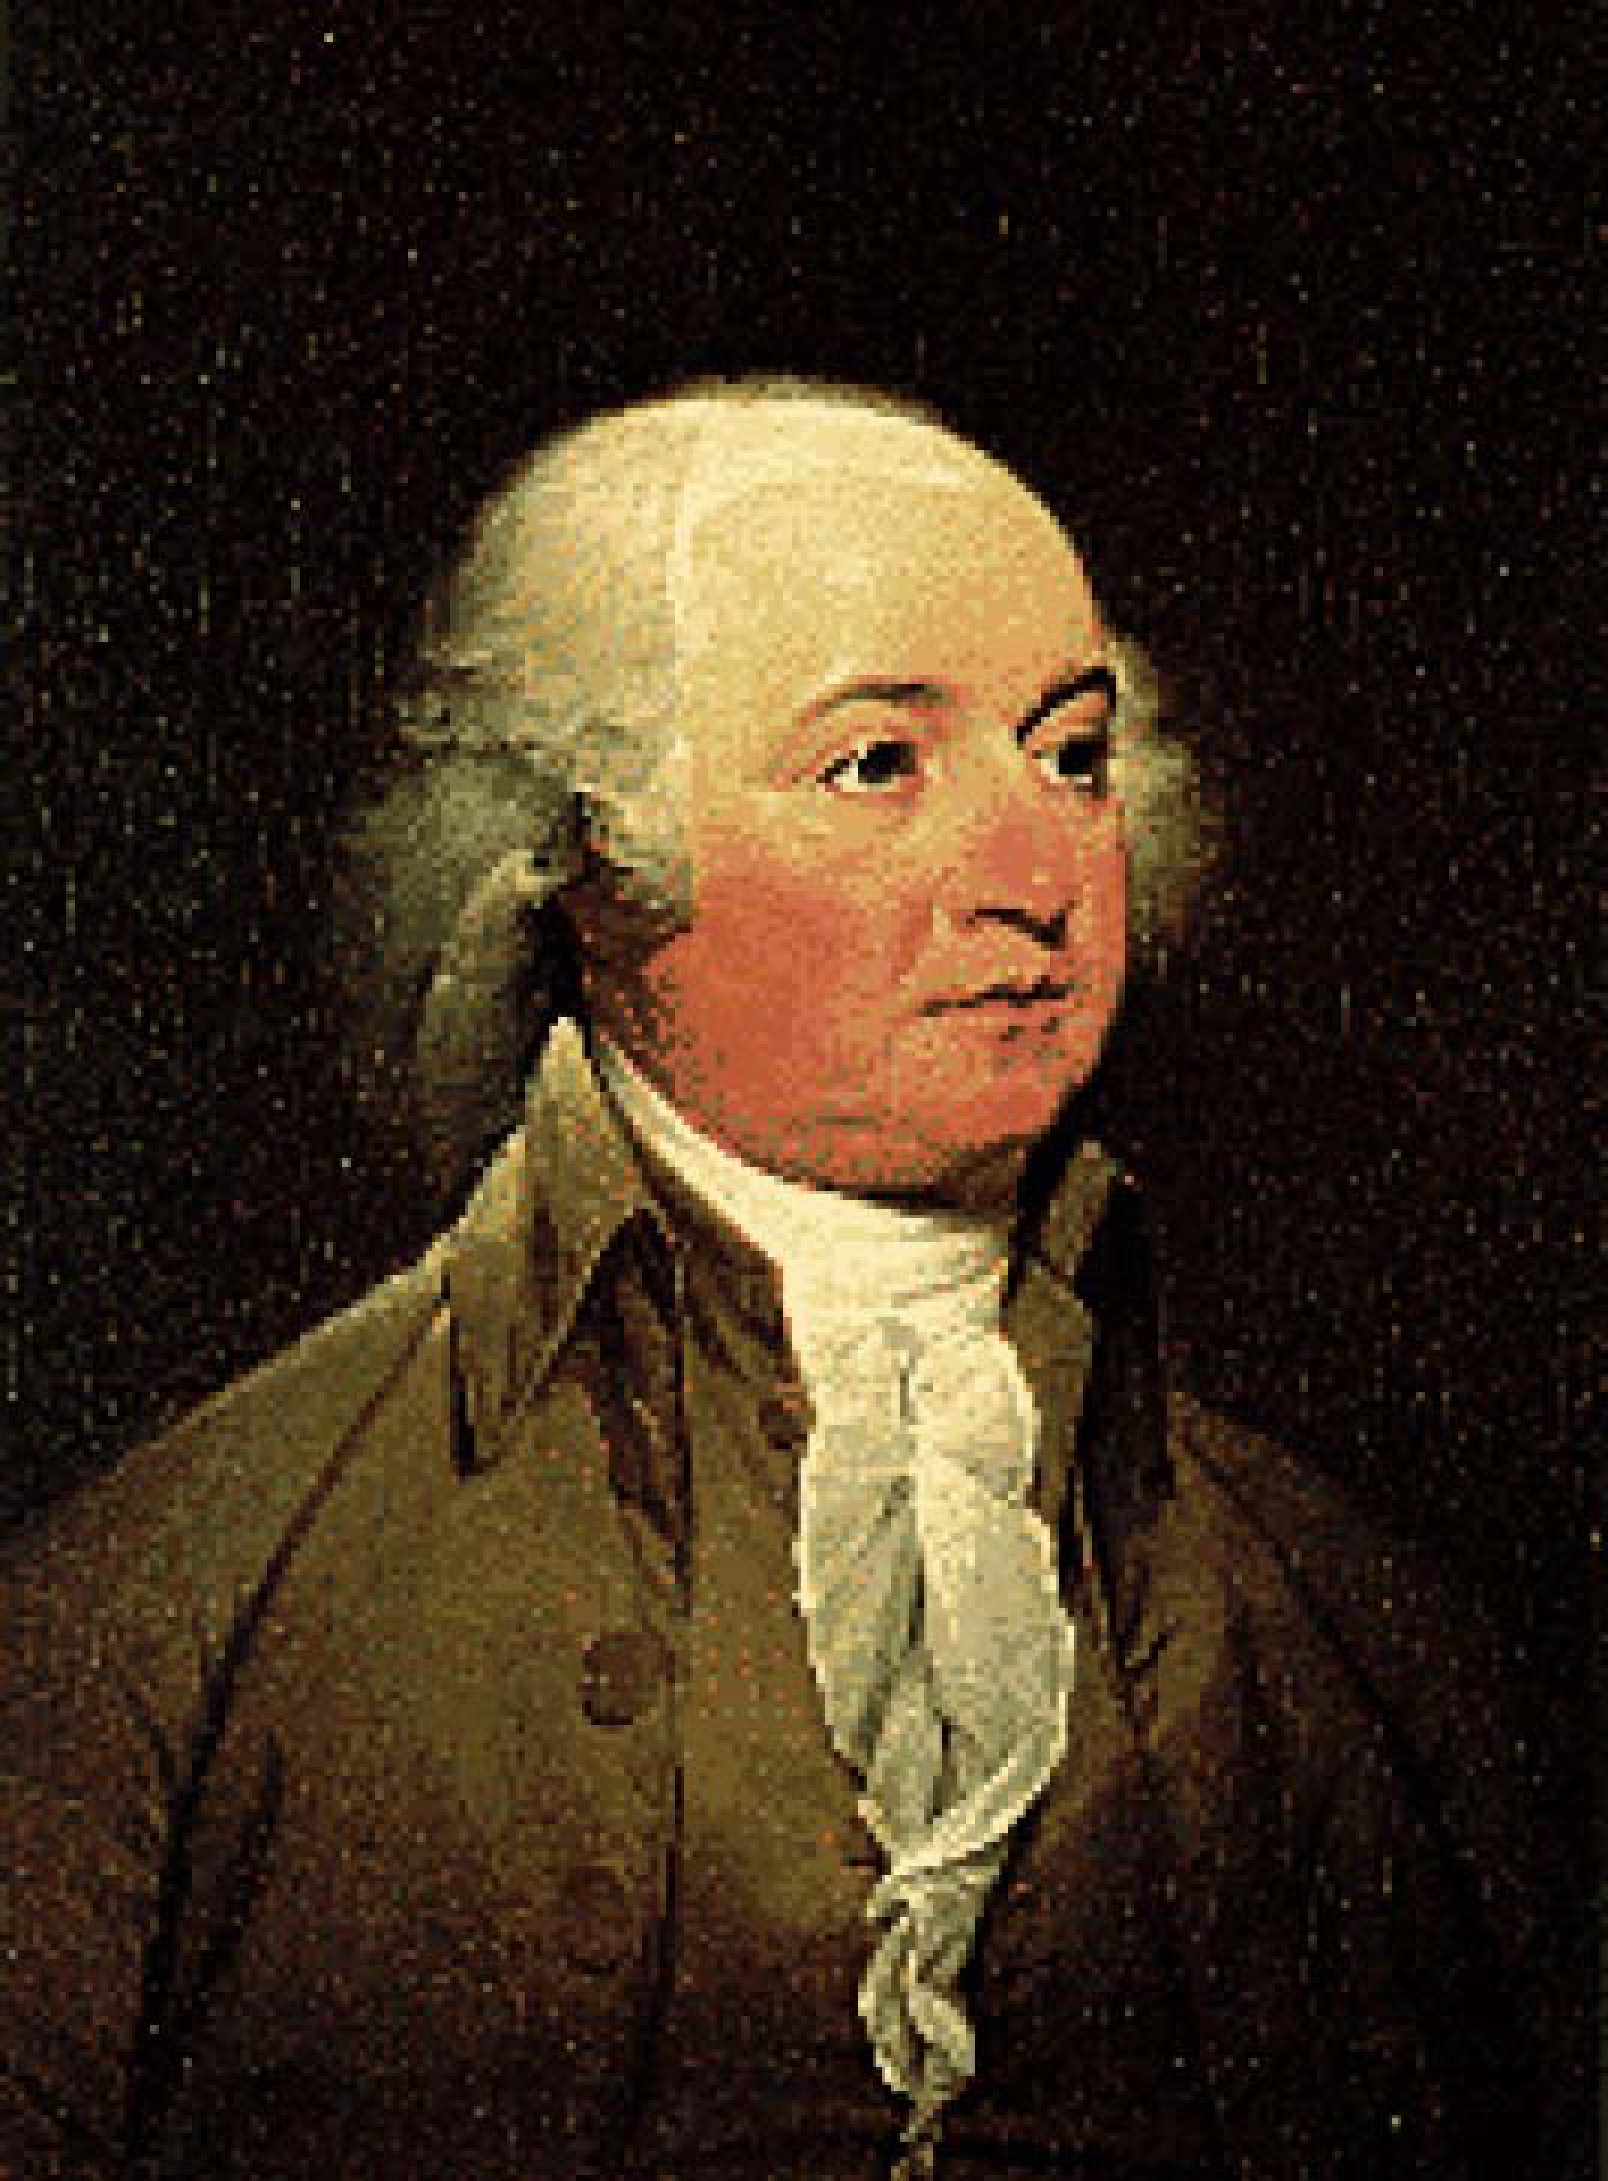
\includegraphics[scale=\rescale]{presidents/ja2}\\
                John Adams\\
                1797-1801
        \fi
        \end{answer}
    \end{response}
\end{card}

% local override
\begin{card}[nohint]
    Who was the third President of the United States?
    \begin{multiChoice}{2}
        \Ans0 Geo. Washington &\Ans0 Ben Franklin \\
        \Ans1 Thomas Jefferson &\Ans0 James Madison
    \end{multiChoice}
    \begin{response}
        \begin{hint}
            He was one of the authors of the Declaration of Independence.
        \begin{multiChoice}{2}
            \Ans0 Geo. Washington &\Ans0 Ben Franklin \\
            \Ans1 Thomas Jefferson &\Ans0 James Madison
        \end{multiChoice}
        \end{hint}
        \begin{answer}
        \ifecListing
            Thomas Jefferson (1801-1809)
        \else\centering
            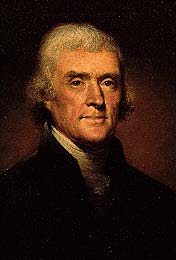
\includegraphics[scale=\rescale]{presidents/tj3}\\
                Thomas Jefferson\\
                1801-1809
        \fi
        \end{answer}
    \end{response}
\end{card}

% this cards should have a hint, since \useHints is now the default
\begin{card}
    \raggedright Who was the fourth President of the United States? \ifecListing\newline\fi
    \begin{fillIn}
    \RespBoxTxt{0}{0}{2}{James Madison}{Madison}
    \end{fillIn}
    \begin{response}
        \begin{hint}\raggedright
            He coauthored the \textsl{Federalists Essays} along with
            John Jay and Alexander Hamilton.
        \begin{fillIn}
            \RespBoxTxt{0}{0}{2}{James Madison}{Madison}
        \end{fillIn}
        \end{hint}
        \begin{answer}
        \ifecListing
            James Madison (1809-1817)
        \else\centering
            \includegraphics[scale=\rescale]{presidents/jm4}\\
            James Madison\\
            1809-1817
        \fi
        \end{answer}
    \end{response}
\end{card}

% back to ho hints as the default
\useNoHints

\begin{card}
    Who was the fifth President of the United States?
    \begin{response}
        \begin{hint}
            In foreign affairs, this President proclaimed a doctrine that
            bears his name, ``\dots the American continents'', he stated, ``by the
            free and independent condition which they have assumed and
            maintain, are henceforth not to be considered as subjects for
            future colonization by any European Power.''
        \end{hint}
        \begin{answer}
        \ifecListing
            James Monroe (1817-1825)
        \else\centering
            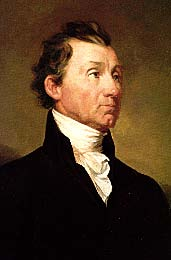
\includegraphics[scale=\rescale]{presidents/jm5}\\
            James Monroe\\
            1817-1825
        \fi
        \end{answer}
    \end{response}
\end{card}

% local override
\begin{card}[hint]
    Who was the sixth President of the United States?
    \begin{response}
        \begin{hint}
            He was the first President who was the son of a President.
        \end{hint}
        \begin{answer}
        \ifecListing
            John Quincy Adams (1825-1829)
        \else\centering
            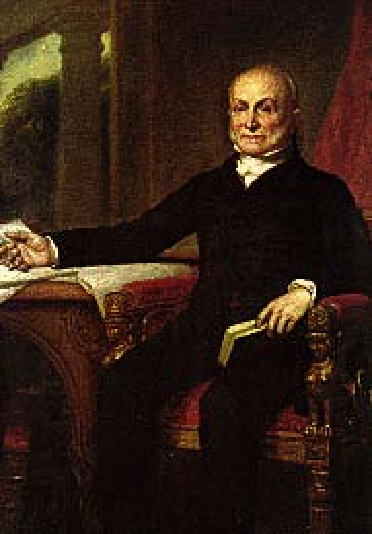
\includegraphics[scale=\rescale]{presidents/ja6}\\
            John Quincy Adams\\
            1825-1829
        \fi
        \end{answer}
    \end{response}
\end{card}

\end{document}
